\chapter{Low value and 2-connected components}

\section{Low value}

For a vertex $v$, $\mathrm{low}(v)$ is the smallest discovery time, $\mathrm{disc}(x)$, over all vertices which can be reached from $v$ using tree edges (away from root) -- red edges -- and at most one back edge -- black edge.

In the example below labels of vertices are (vertex name, discovery time, low value) and arrows indicate parent of a vertex (prev).

\begin{center}
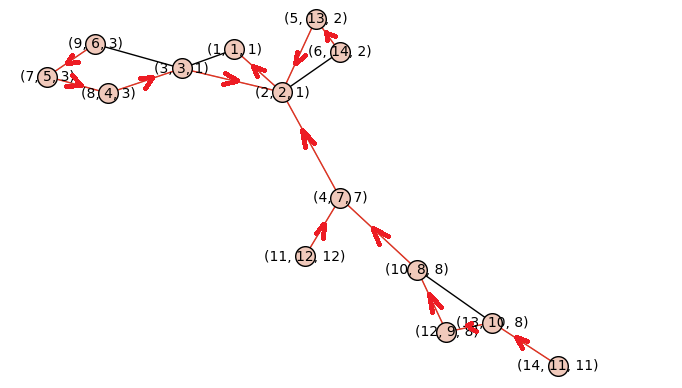
\includegraphics[width=0.9\textwidth]{Images/Low/low.png}
\end{center}

$\mathrm{low}(2)$ is $1$ since we can reach the root (with discovery time $1$) using red edge $(2, 3)$ and black edge $(3, 1)$.

$\mathrm{low}(8)$ is $3$ since the vertex with the smallest discovery time we can reach in the prescribed way is $3$: edges are $(8, 7), (7, 9), (9, 3)$ and $3$ has discovery time $3$.

$\mathrm{low}(10)$ is $8$ (its discovery time) since we can not reach any vertex with smaller discovery time using the tree edges "below" $10$.

\medskip
Use a recursive implementation of the depth-first search given in the previous chapter to compute the low value of each vertex in a graph.

\medskip
\begin{sageCell}
def DFS_low(G, r):
    """
    Calculate DFS with root r, discovery time, low values.
    """
    global time
    time = 0
    prev = {}
    disc = {}
    low = {}
    prev[r] = None
    DFS_low_call(G, r, prev, disc, low)
    return (prev, disc, low)

def DFS_low_call(G, v, prev, disc, low):
    global time
    time += 1;
    disc[v] = time;
    low[v] = time;
    for u in G.neighbors(v):
        if u not in prev:
            prev[u] = v
            DFS_low_call(G, u, prev, disc, low)
    for u in G.neighbors(v):
        if prev[u] == v:
            # edge (vertex) in "subtree"
            low[v] = min(low[v], low[u])
        elif u != prev[v]:
            # "back edge" and not a tree edge
            low[v] = min(low[v], disc[u])
\end{sageCell}

\subsubsection*{Example}

\begin{sageCell}
    G = Graph({1:[2,3], 2:[3,4,5,6], 3:[8,9], 4:[10,11], 5:[6], 7:[8,9],
    10:[12,13], 12:[13], 13:[14]})
    (prev, disc, low) = DFS_low(G, 1)
    low
\end{sageCell}
\begin{outCell}
    {1: 1,
     2: 1,
     3: 1,
     8: 3,
     7: 3,
     9: 3,
     4: 7,
     10: 8,
     12: 8,
     13: 8,
     14: 11,
     11: 12,
     5: 2,
     6: 2}
\end{outCell}

Relabel vertices with triples (vertex label, discovery time, low value) and color tree edges red

\begin{sageCell}
    G1 = G.relabel(dict([(v, (v, disc[v], low[v])) for
        v in G.vertices(sort=False)]), inplace=False)
    G1.plot(edge_colors={'red': [((u, disc[u], low[u]), (v, disc[v],
        low[v])) for (u, v) in prev.items() if v != None]})
\end{sageCell}
\begin{outImage}
    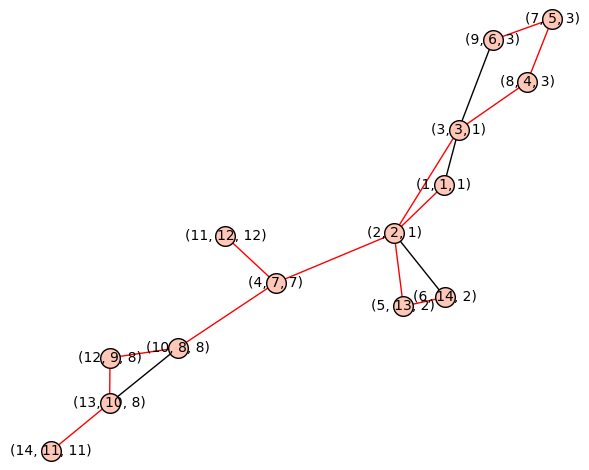
\includegraphics[width=0.9\textwidth]{Images/Low/output_low.png}
\end{outImage}

\section{Cutvertices}

We can get cutvertices using the following Theorem:

\begin{theorem}
Let $G$ be connected, undirected, simple, let $r$ be the root of its DFS tree $T$:
\begin{itemize}
\item $r$ is a cutvertex if it is incident with at least $2$ tree edges
\item nonroot vertex $v$ is a cutvertex if $v$ has a son $y$ so that $\mathrm{low}(y) \geq \mathrm{disc}(v)$
\end{itemize}
\end{theorem}

In the example above, cutvertices are $2, 3, 4, 10, 13$. For example, $10$ is a cutvertex, since its son in the tree has low value $8$ which is $\geq$ than discovery time of $10$, which is $8$.

Also, $4$ is a cutvertex since its sons ($11$ and $10$) have low values $\geq 7$
($7 = \mathrm{disc}(4)$).

The root $1$ is not a cutvertex since it is incident with only one tree edge.

\medskip
\begin{sageCell}
def cutvertices(G):
    """
    Retuns an array of cutvertices of a connected graph G.
    """
    root = G.vertices(sort=False)[0]     # assume G is connected
    (prev, start, low) = DFS_low(G, root)
    result = []
    rootn = 0
    for v in G.vertices(sort=False):
        for u in G.neighbors(v):
            if v != root:
                if v == prev[u] and low[u] >= start[v]:
                    result.append(v)
                    break
            elif v == prev[u]:
                rootn += 1
    if rootn >= 2:
        result.append(root)
    return result
\end{sageCell}

\subsubsection*{Example}

\begin{sageCell}
    cutvertices(G)
\end{sageCell}
\begin{outCell}
    [2, 3, 4, 13, 10]
\end{outCell}

\begin{sageCell}
    plot(G, vertex_colors={'red': cutvertices(G)})
\end{sageCell}
\begin{outImage}
    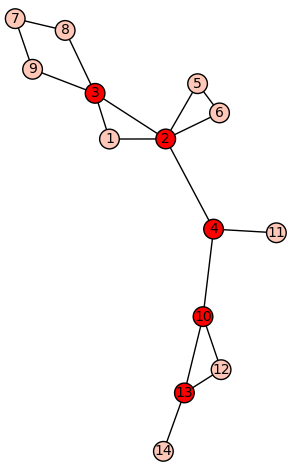
\includegraphics[width=0.45\textwidth]{Images/Low/output_cutvertices.png}
\end{outImage}

\section{2-connected components}

Write a function partition(G) which partitions edges of G into blocks (2-connected components).

Output should be a dictionary which maps an edge of the graph into a number which represents a block. In the example above, vertices $1, 2, 3$ (edges $(1,2), (1,3), (2,3)$) create a block. Therefore the resulting dictionary should map the pairs $(1,2), (1,3), (2,3)$ into the same number, say $1$.

\medskip
\begin{sageCell}
def partition(G):
    """"
    Partitions of edges of a connected graph G into blocks.
    Returns a dictionary mapping each edge to the block (number) it belongs to.
    """
    global blocknum
    root = G.vertices(sort=False)[0]     # assume G is connected
    (prev, start, low) = DFS_low(G, root)
    blocknum = 0
    blocks = {}
    partition_call(G, root, prev, start, low, blocks, 0)
    return blocks

def partition_call(G, v, prev, start, low, blocks, blockn):
    global blocknum
    for u in G.neighbors(v):
        if v == prev[u]: # forward tree edge
            if low[u] >= start[v]: # cut vertex, start a new block
                blocknum += 1
                blocks[(v, u)] = blocknum
                partition_call(G, u, prev, start, low, blocks, blocknum)
            else: # stay in the same block
                blocks[(v, u)] = blockn
                partition_call(G, u, prev, start, low, blocks, blockn)
        elif start[u] < start[v] and u != prev[v]: # back edge not in tree
            blocks[(u, v)] = blockn
\end{sageCell}

\subsubsection*{Example}

\begin{sageCell}
    partition(G)
\end{sageCell}
\begin{outCell}
    {(10, 4): 1,
     (4, 2): 2,
     (2, 1): 3,
     (1, 3): 3,
     (2, 3): 3,
     (3, 8): 4,
     (8, 7): 4,
     (7, 9): 4,
     (3, 9): 4,
     (2, 5): 5,
     (5, 6): 5,
     (2, 6): 5,
     (4, 11): 6,
     (10, 12): 7,
     (12, 13): 7,
     (10, 13): 7,
     (13, 14): 8}
\end{outCell}

\begin{sageCell}
import random
def edge_colors(part):
    blocks = set(part.values())
    colors = [(random.random(), random.random(), random.random()) for b in blocks]
    colorblocks = [[edge for edge in part.keys() if part[edge] == b] for b in blocks]
    return dict(zip(colors, colorblocks))
\end{sageCell}
\begin{sageCell}
    G.plot(edge_colors=edge_colors(partition(G)))
\end{sageCell}
\begin{outImage}
    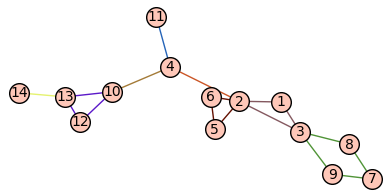
\includegraphics[width=0.6\textwidth]{Images/Low/output_partition.png}
\end{outImage}
